\subsection{Mejorando la complejidad espacial: Matrices ralas}
\label{sec:ralas}

Para realizar el \textit{clustering} es necesario primero generar una matriz de
distancias entre tractogramas. Por ello es conveniente tener todos 
los tractogramas en memoria. En nuestro caso, la matriz con los \textbf{tractogramas
sin transformar} del \'Area de Broca tiene dimensiones $762\times3587328$. 
Asumiendo que cada valor se representa usando $8$ Bytes, esta matriz ocupa un 
total de aproximadamente $20$ Gigabytes. Sin embargo, solo un $1\%$ de los datos
almacenados son no nulos. Esto implica que casi todo el espacio utilizado es
desperdiciado. \\

Es posible mejorar esto eliminando de la matriz las columnas que poseen solo
elementos nulos. La Figura \ref{fig:densa} muestra la matriz que resulta de
eliminar las columnas vacias de la matriz del \'Area de Broca. Si bien la nueva
matriz posee dimensiones $762\times121045$, a\'un solo el $27\%$ de los valores 
almacenados son no nulos. Manteniendo la representaci\'on de $8$ Bytes es posible
reducir el espacio necesario de $20$ Gigabites a aproximadamente $700$ Megabytes.\\

\begin{figure}[h!]
   \centering
    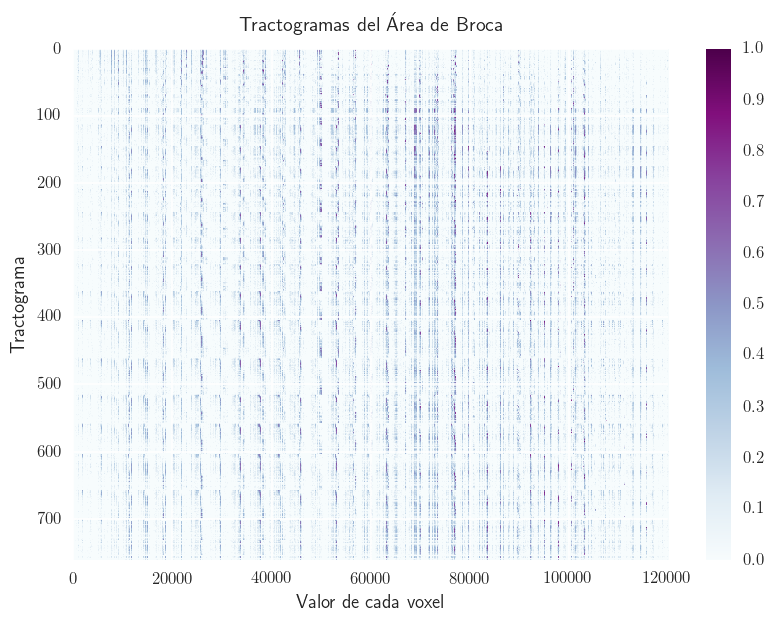
\includegraphics[width=0.9\textwidth]{img/densa_broca.png}
    \caption{Semillas en el hemisferio izquierdo. }
    \label{fig:densa}
\end{figure}

El problema de este \'ultimo m\'etodo es que a\'un desperdicia mucho espacio. En
el caso de utilizar todas los \textbf{tractogramas sin transformar} de un 
hemisferio, la matriz pasa a ser de dimensiones $21657\times3587328$ con un $1\%$
de valores no nulos. Para almacenar dicha matriz es necesario utilizar $587$ 
Gigabytes. Por esto es necesario utilizar estructuras mas eficiente, que aprovechen
lo ralo de las matrices. Ejemplos de estas estructuras son: \textit{Dictionary of
Keys}, o una matriz \textit{Compressed Sparse Row} (CSR). \\

%eliminando columnas in\'utiles nos queda 21657x145574, son 23.5 Gn

Si recordamos la forma que tiene la funci\'on logit encontramos un inconveniente
al querer utilizar matrices ralas. Podemos ver en la Figura \ref{fig:dominio} que
\textit{logit}$(0) = -\infty$. Esto implica que la transformaci\'on de una matriz
rala no es rala en t\'erminos de elementos nulos. Sin embargo podemos aprovechar
ciertas propiedades para recuperar las matrices ralas. La distancia euclidena 
entre vectores es invariante a traslaciones lineales del sistema. Lo mismo sucede
con las posiciones relativas de los centroides. Asignemos una representaci\'on 
finita $c$ al valor $-\infty$. Un buen candidato para $c$ es el $log(\epsilon)$,
donde $\epsilon$ es el \textit{epsilon de la maquina}. Transformar todos los vectores
y luego trasladarlos sumando $c$ en cada componente dara como resultado una
representaci\'on rala. Gracias a esto podemos utilizar DOK, CSR o cualquier
estructura para reducir los costos espaciales de almacenar los tractogramas. \\

Existen maneras eficientes de multiplicar matrices ralas entre si \cite{Bank1993}.
Si calculamos la distancia euclidea entre dos vectores ralos usando la siguiente
relaci\'on: 

\begin{equation}
\label{eq:simileuc}
simil_{euc}(X,Y) = \sqrt{X \cdot X^t - 2 X \cdot Y^t + Y \cdot Y^t} 
\end{equation}
Podemos generar la matriz de distancias usando directamente las estructuras de 
matrices ralas. Es importante destacar que este m\'etodo generara una matriz que no 
necesariamente es sim\'etrica. Algunos valores que deber\'ian ser iguales pueden
presentar un peque\~no error num\'erico.
